\newcommand{\langue}{french}
% Préambule commun aux rapports. Définir \langue (french ou english) avant de l'inclure.
\documentclass[10pt,a4paper,twocolumn]{article}
\usepackage[T1]{fontenc}
\usepackage[utf8]{inputenc}
\usepackage{lmodern}
\usepackage[\langue]{babel}
\usepackage[a4paper,hmargin=1.5cm,top=1.5cm,bottom=2cm]{geometry}
\usepackage{amsmath,amssymb,graphicx,booktabs,enumitem,microtype}
\usepackage[font=small,skip=6pt]{caption}
\usepackage[hidelinks]{hyperref}
\setlength{\columnsep}{0.85cm}
\setlist{leftmargin=1.2em,itemsep=1pt,topsep=3pt,parsep=0pt}
\newcommand{\pa}[1]{\par\smallskip\noindent\textbf{#1}\enspace}
\newcommand{\ket}[1]{\lvert #1\rangle}
\newcommand{\en}[1]{\emph{#1}}
% \entete{titre}{sous-titre}{cadre}{auteurs et lignes suivantes}{nom du résumé}{résumé}
\newcommand{\entete}[6]{%
\twocolumn[\begin{center}
{\LARGE\bfseries #1\par}\vspace{6pt}
{\large #2\par}\vspace{10pt}
{\large\bfseries #3\par}\vspace{2pt}
{#4\par}
\end{center}
\vspace{4pt}
\begin{center}\begin{minipage}{0.9\textwidth}
\begin{center}\bfseries #5\end{center}\vspace{-4pt}
\small #6
\end{minipage}\end{center}
\vspace{14pt}]}
\frenchspacing
\raggedbottom

\hypersetup{pdftitle={Robot mobile autonome pour la capture de balises},pdfauthor={Eliott Dionnet}}
\begin{document}
\entete{Robot Mobile Autonome pour la Capture de Balises}
{Asservissement des moteurs, localisation par marqueurs ArUco\\ et planification à plusieurs robots}
{Rapport de Projet -- Artefact (PROJ103)}
{Télécom Paris, 2024--2025, \textsc{Dionnet Eliott}\\
Avec la contribution de \textsc{Cordelle Alexis}, \textsc{Boudouh Mohamed} et \textsc{Palagi Théo}\\
11 novembre 2026}
{Résumé}
{Ce rapport décrit un robot mobile qui parcourt une arène quadrillée pour y repérer et capturer des balises
portant des marqueurs ArUco, piloté à distance, puis autonome, enfin au sein d'une stratégie commune à
plusieurs robots. Le robot repose sur une Raspberry Pi, une carte de commande des moteurs pilotée en I\textsuperscript{2}C et
une caméra. Les déplacements sont asservis par un correcteur PID sur les encodeurs des roues : le robot avance
par pas de 50~cm et tourne par multiples de 45°. La caméra, calibrée sur 35 images de damier avec une erreur
de reprojection moyenne de 0,37~pixel, donne la pose de chaque marqueur détecté. Pour l'épreuve finale, le
groupe a modélisé l'arène par un graphe de 336 états, sur lequel une recherche exhaustive s'est révélée trop
lente, ce qui a conduit à une stratégie gloutonne guidée par des priorités. Le robot a réussi l'épreuve finale.}

\section{Introduction et Contexte}
Le projet Artefact (PROJ103) de Télécom Paris demande à chaque équipe de construire un robot capable
de se déplacer dans une arène et d'y trouver des balises.
L'arène est un quadrillage de cases de 50~cm. Les balises
portent des marqueurs ArUco~\cite{aruco}, et des marqueurs fixes
sont placés dans les coins. Un serveur du cours reçoit en
continu la position estimée de chaque robot et enregistre
les balises capturées, identifiées par leur numéro et leur case.

Le projet s'est déroulé en trois temps, chacun conclu
par une épreuve : piloter le robot à distance, explorer
l'arène et capturer des balises de façon autonome, puis
participer à une stratégie commune où un serveur coordonne plusieurs robots.

Ce rapport présente l'architecture du robot (section~\ref{s:archi}),
la commande des moteurs (section~\ref{s:moteurs}), la vision (section~\ref{s:vision}),
l'exploration autonome (section~\ref{s:explo}) et la planification à
plusieurs robots étudiée pour l'épreuve finale (section~\ref{s:plan}).

\begin{figure}[t]
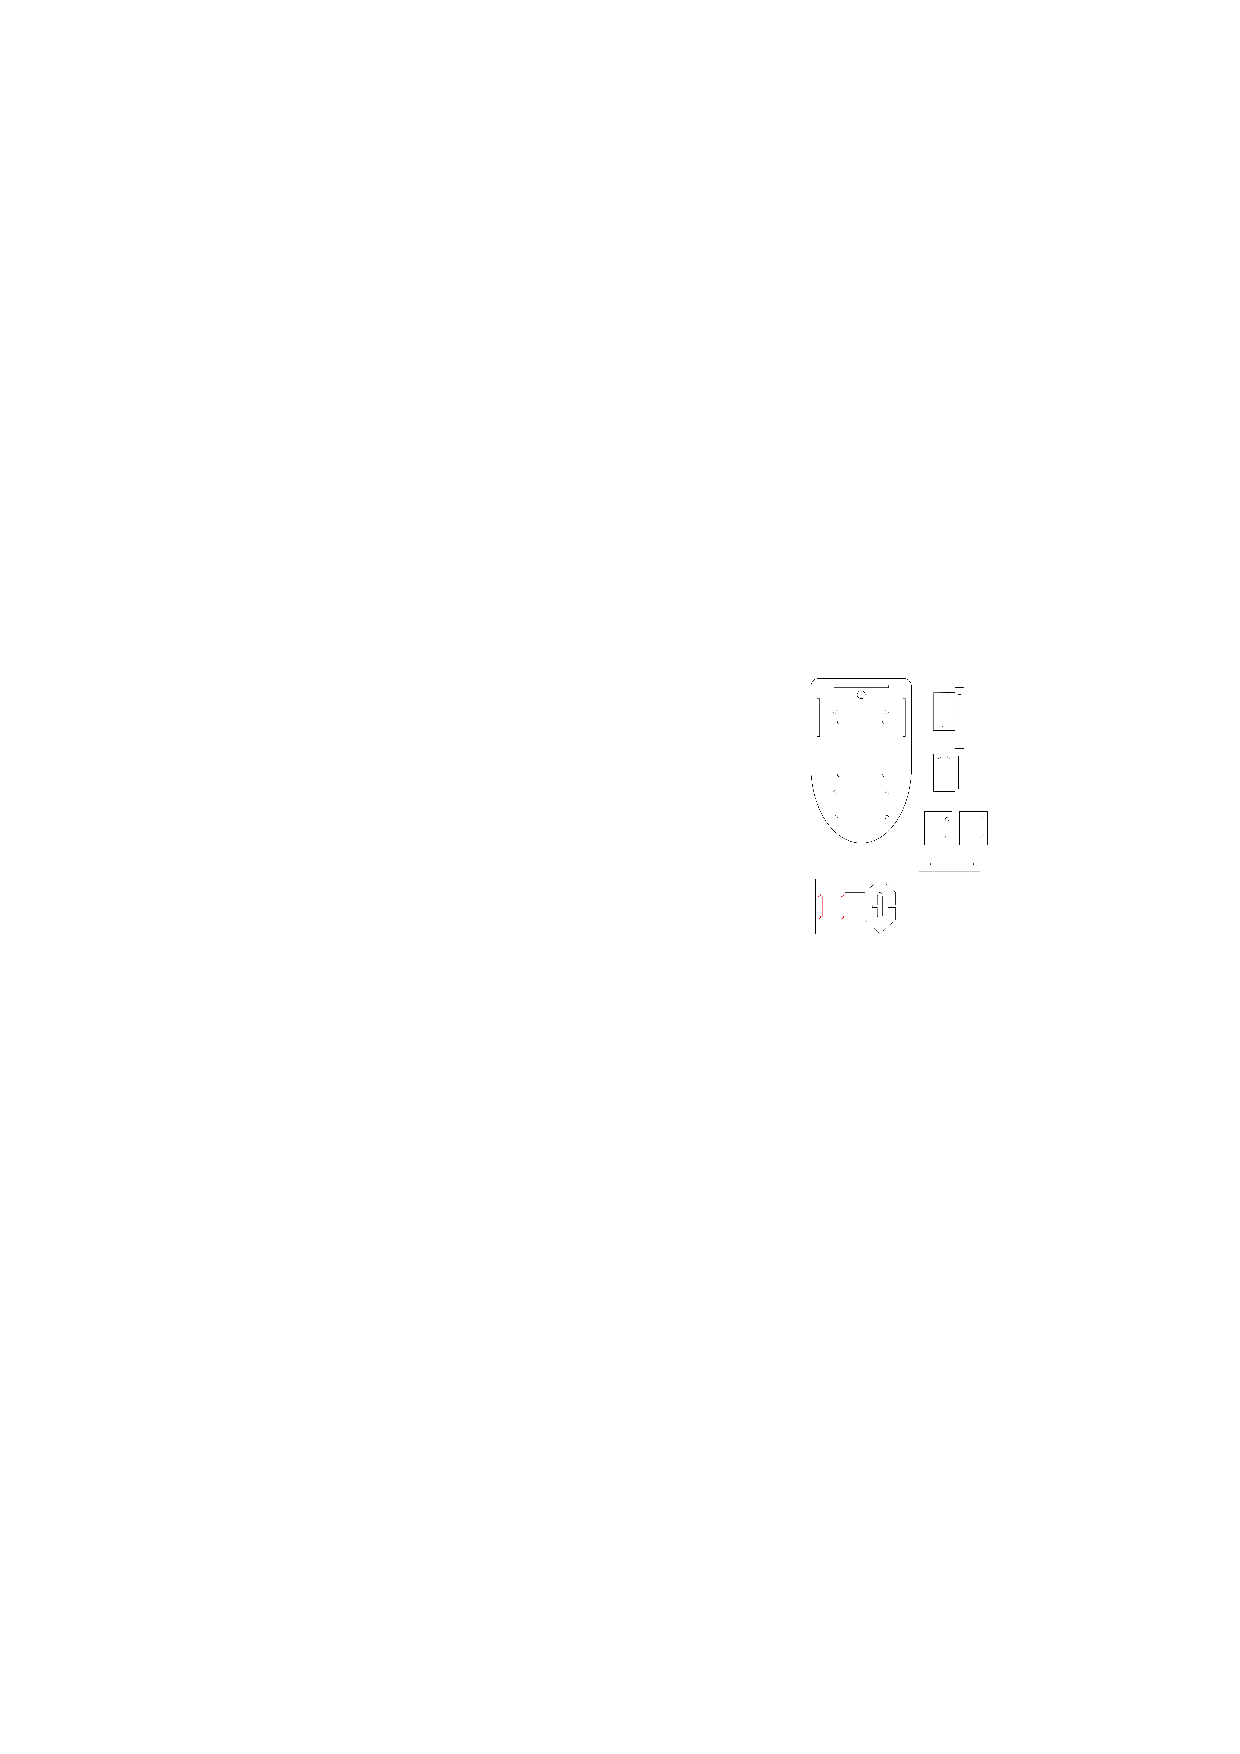
\includegraphics[width=\linewidth]{figs/robot-1}
\caption{Plan de découpe du châssis du robot, dessiné pour le Fablab : la plaque principale,
les supports des moteurs et le support de la caméra.}\label{f:chassis}
\end{figure}

\section{Architecture du Robot}\label{s:archi}
Le châssis a été découpé au Fablab à partir du plan
de la figure~\ref{f:chassis}. Il porte deux roues motrices, une batterie,
une Raspberry Pi et une caméra. La Raspberry Pi communique avec une carte de commande des moteurs par
le bus I\textsuperscript{2}C. Cette carte fixe la vitesse de chaque moteur
et renvoie les \en{ticks} comptés par les encodeurs des roues depuis la dernière lecture.

Tout le logiciel est écrit en Python et partagé par un
dépôt Git, que la Raspberry Pi ne fait que récupérer.
La figure~\ref{f:echanges} résume les échanges entre le robot et son environnement.

\pa{Pilotage manuel.} Pour la première épreuve, le robot
exécute un petit serveur qui reçoit les commandes. Une
page web propose cinq boutons (avancer, reculer, tourner
à gauche ou à droite, s'arrêter), et un programme lit les
axes d'une manette avec la bibliothèque pygame et envoie
par WebSocket la vitesse des deux roues.

\section{Commande des Moteurs}\label{s:moteurs}
\pa{Ligne droite.} Imposer la même consigne aux deux
moteurs ne suffit pas à rouler droit, car les deux moteurs ne réagissent pas exactement de la même façon. Le
programme d'avance mesure donc à chaque pas de 0,1~s
l'écart cumulé entre les \en{ticks} des deux roues, $e = N_d - N_g$,
et corrige les vitesses par un PID~\cite{astrom} :
\begin{equation}
u = K_p\,e + K_i \sum e + K_d\,\Delta e, \qquad v_{g,d} = v_0 \pm u,
\end{equation}
avec $K_p = 0{,}035$, $K_i = K_d = 0{,}025$ et une vitesse de base
$v_0 = 50$. Le terme intégral est borné pour éviter qu'il ne
s'emballe quand la correction sature. Le robot s'arrête
quand la moyenne des \en{ticks} atteint la cible, à raison
de 206 \en{ticks} par centimètre. Un facteur de 0,86 sur la
distance demandée, ajusté expérimentalement, compense
le dépassement à l'arrêt.

\begin{figure}[t]
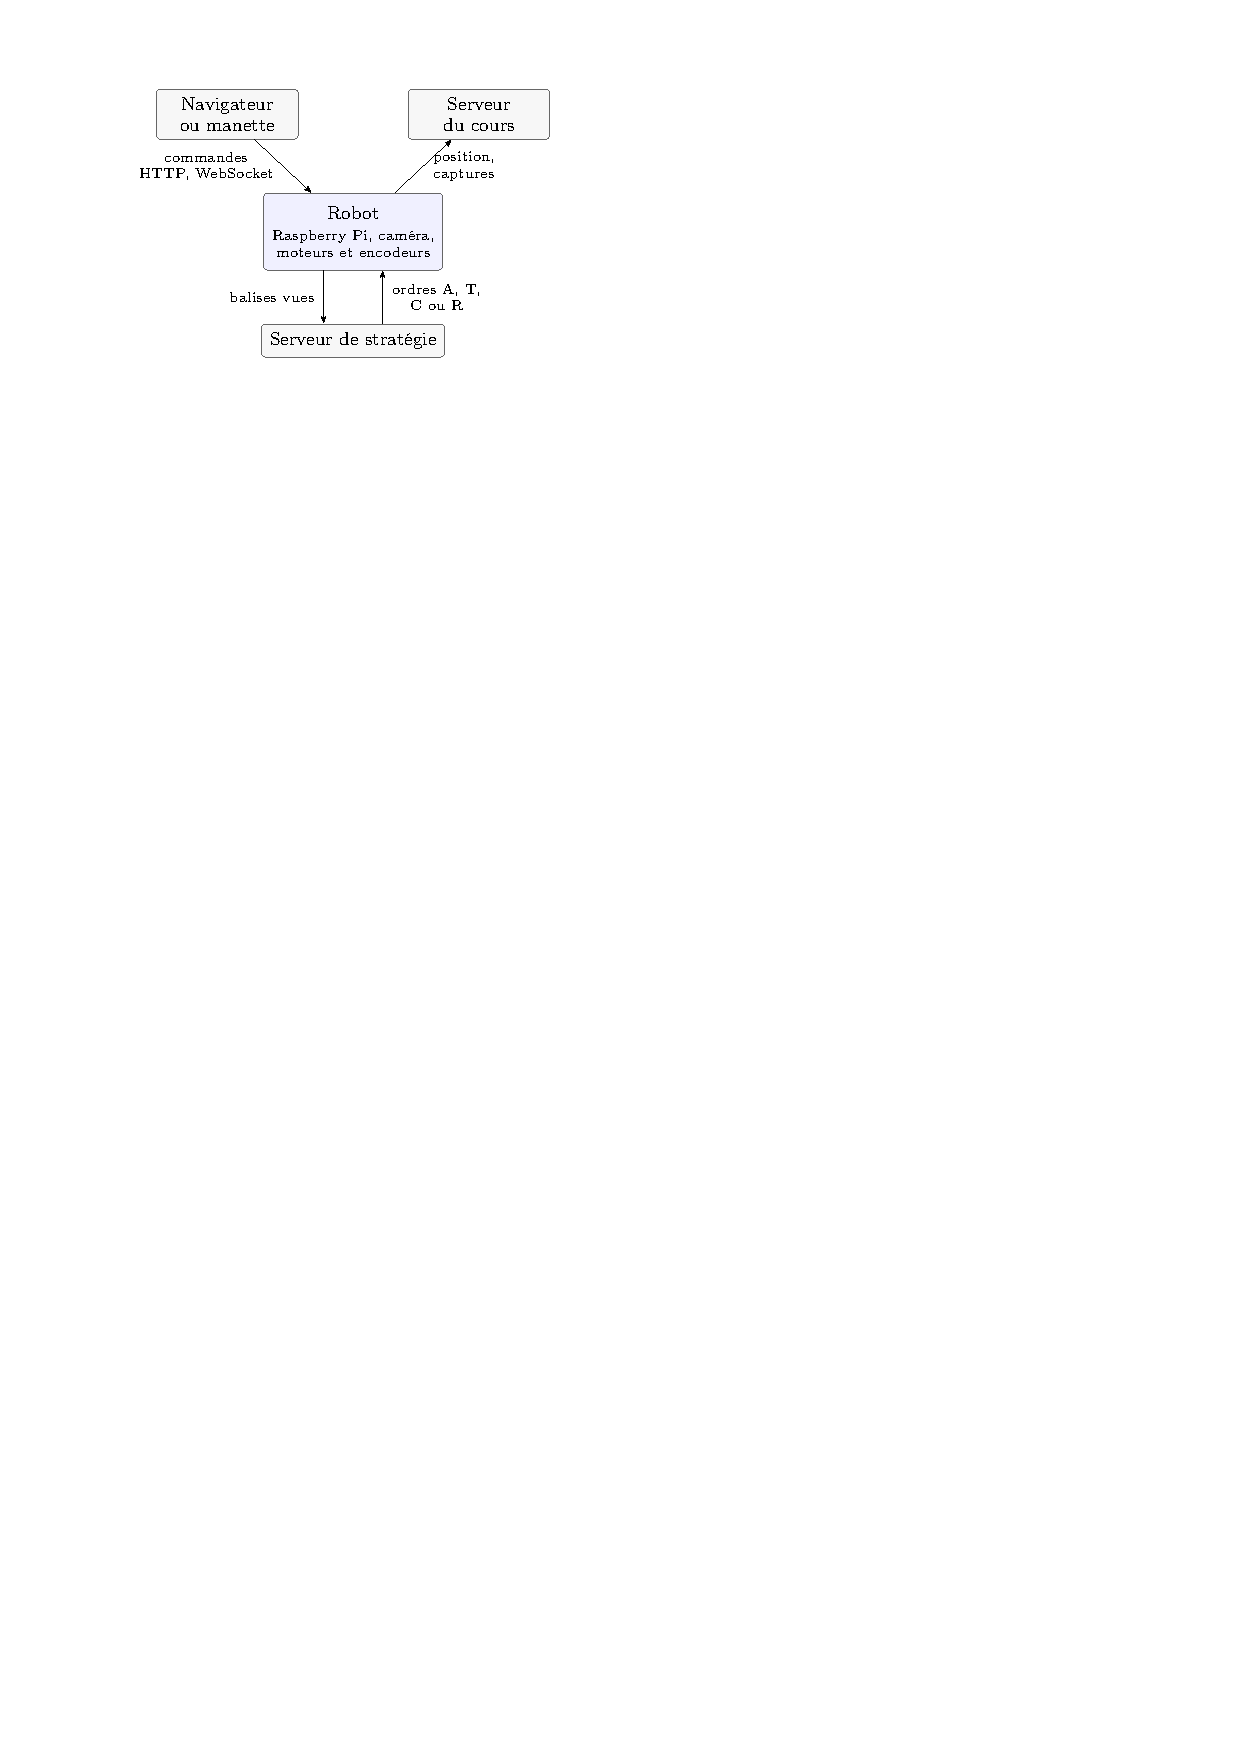
\includegraphics[width=\linewidth]{figs/robot-2}
\caption{Échanges du robot. Le pilotage manuel passe
par HTTP ou par WebSocket. Le serveur du cours reçoit la
position et les captures. Pour l'épreuve finale, un serveur de
stratégie reçoit les balises vues et renvoie des ordres.}\label{f:echanges}
\end{figure}

\pa{Rotation.} Pour tourner sur place, l'erreur devient
l'écart entre la cible, à raison de 55,2 \en{ticks} par degré,
et la différence des \en{ticks} des deux roues. Le même correcteur pilote alors des vitesses opposées, plafonnées pour
limiter le dépassement. La rotation s'arrête quand l'erreur passe sous 10 \en{ticks}, soit environ 0,2°, ou quand elle
ne bouge plus pendant 20 pas.

\pa{Odométrie.} La position du robot est tenue à jour à
partir des ordres exécutés : chaque avance de 50~cm
déplace le robot d'une case dans la direction courante, et
chaque rotation met à jour son cap. Cette estimation est
envoyée au serveur du cours chaque seconde. Elle suppose
des déplacements parfaits : l'erreur s'accumule au fil des
mouvements, ce qui motive le recalage par la caméra.

\section{Vision}\label{s:vision}
\pa{Calibration.} La caméra a été calibrée par la méthode
de Zhang~\cite{zhang}, avec OpenCV~\cite{opencv}, sur 35 images d'un damier de $6 \times 4$ coins intérieurs et de cases de 12~mm,
prises en $640 \times 480$. En refaisant la calibration sur ces
images, le damier est retrouvé dans les 35 images et
l'erreur de reprojection vaut 0,58~pixel en moyenne quadratique, 0,37~pixel en moyenne par image (figure~\ref{f:calib}). Une
seule image dépasse 1~pixel. La focale obtenue, environ
1\,335 pixels, correspond à un champ horizontal d'environ
27° : la caméra voit loin, mais étroit.

\begin{figure}[t]
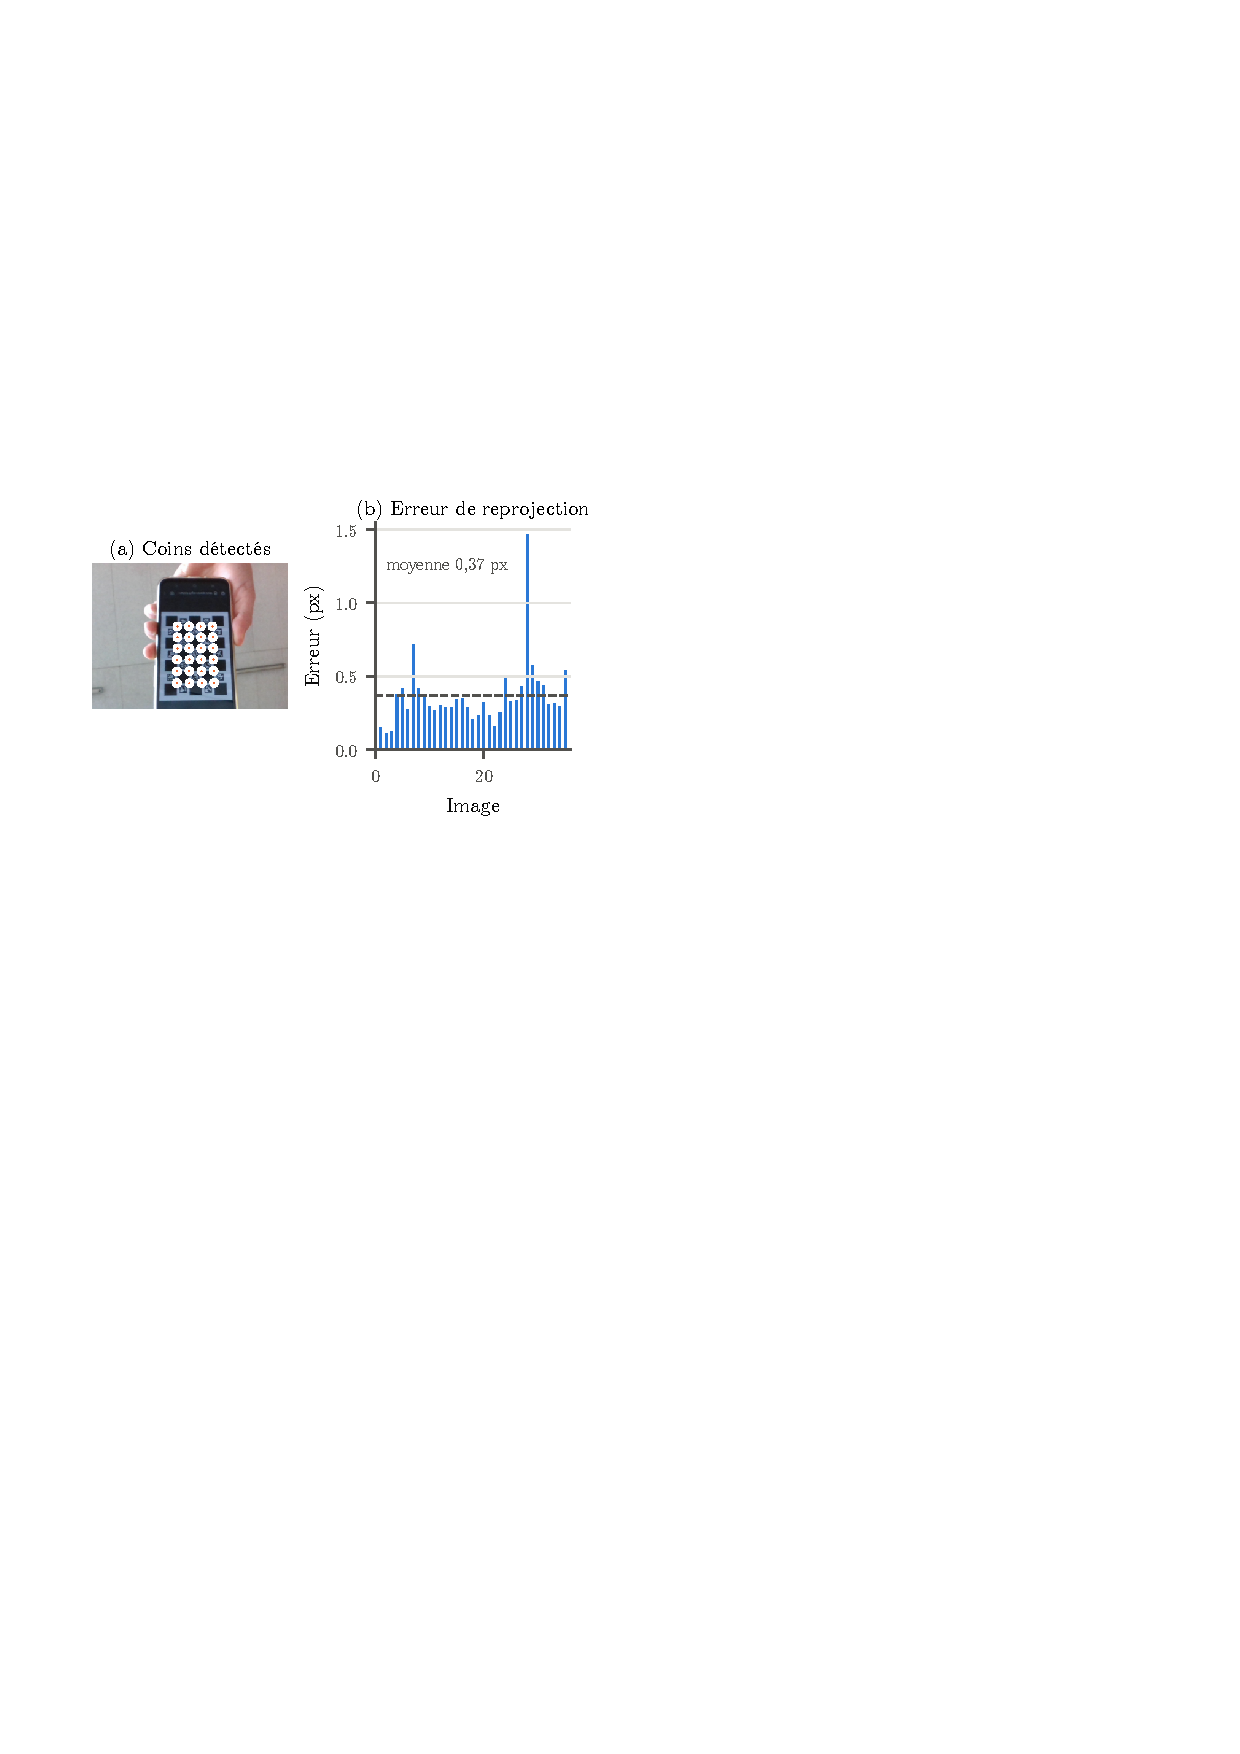
\includegraphics[width=\linewidth]{figs/robot-3}
\caption{Calibration de la caméra. (a) Coins du damier
détectés sur l'une des 35 images. (b) Erreur de reprojection
moyenne de chaque image, calculée en refaisant la calibration
sur les images du projet.}\label{f:calib}
\end{figure}

\pa{Pose des marqueurs.} Les marqueurs sont cherchés
dans le dictionnaire ArUco $6 \times 6$. Pour chaque marqueur
détecté, ses quatre coins et sa taille connue de 10~cm
permettent de résoudre le problème \en{Perspective-n-Point} (PnP),
qui donne sa position $\mathbf{t}$ et son orientation $\mathbf{r}$ dans le
repère de la caméra. La norme de $\mathbf{t}$ donne directement la distance.

\pa{Localisation.} Quand un marqueur de coin est visible,
la transformation inverse donne la position de la caméra
dans le repère du marqueur. Une rotation propre à chaque
coin ramène ensuite cette position dans le repère de
l'arène. Si plusieurs coins sont visibles, le programme fait
la moyenne des estimations. Une première approche, plus
simple, reliait la distance à un marqueur à sa hauteur
apparente en pixels, mesurée tous les 10~cm sur 1,50~m.

\section{Exploration Autonome}\label{s:explo}
Pour la deuxième épreuve, le robot explore l'arène
seul. À chaque case, il effectue un balayage depuis le
centre : une rotation de 45°, puis de 20° supplémentaires
de chaque côté, avec une photographie à chaque arrêt.
Avec un champ d'environ 27°, ces quatre prises de vue
couvrent de 30 à 80° environ de chaque côté du robot.
Les marqueurs de coin, d'identifiants 1 à 4, servent à la
localisation et sont ignorés pendant ce balayage. Un marqueur d'identifiant 0 est noté comme balise potentielle, à
vérifier plus tard.

Quand une vraie balise est détectée, le robot la capture :
il fait un tour complet sur lui-même, puis envoie au
serveur du cours le numéro de la balise et sa case. La
case se déduit de la position estimée, en divisant les
coordonnées par la taille d'une case ; les lignes sont notées
de A à G et les colonnes numérotées à partir de 1. Le
robot revient ensuite à son orientation de départ pour poursuivre.

\section{Planification à Plusieurs Robots}\label{s:plan}
Pour l'épreuve finale, les robots du groupe collaborent.
Un serveur de stratégie reçoit les balises vues par chaque
robot et lui renvoie un ordre parmi quatre : avancer d'une
case (A), tourner d'un angle donné (T), capturer une
balise (C) ou attendre (R). Le robot exécute l'ordre, met
à jour sa position et renvoie ses observations. Tout le
calcul de la stratégie est donc centralisé. Ce travail a été mené en groupe.

\begin{figure}[t]
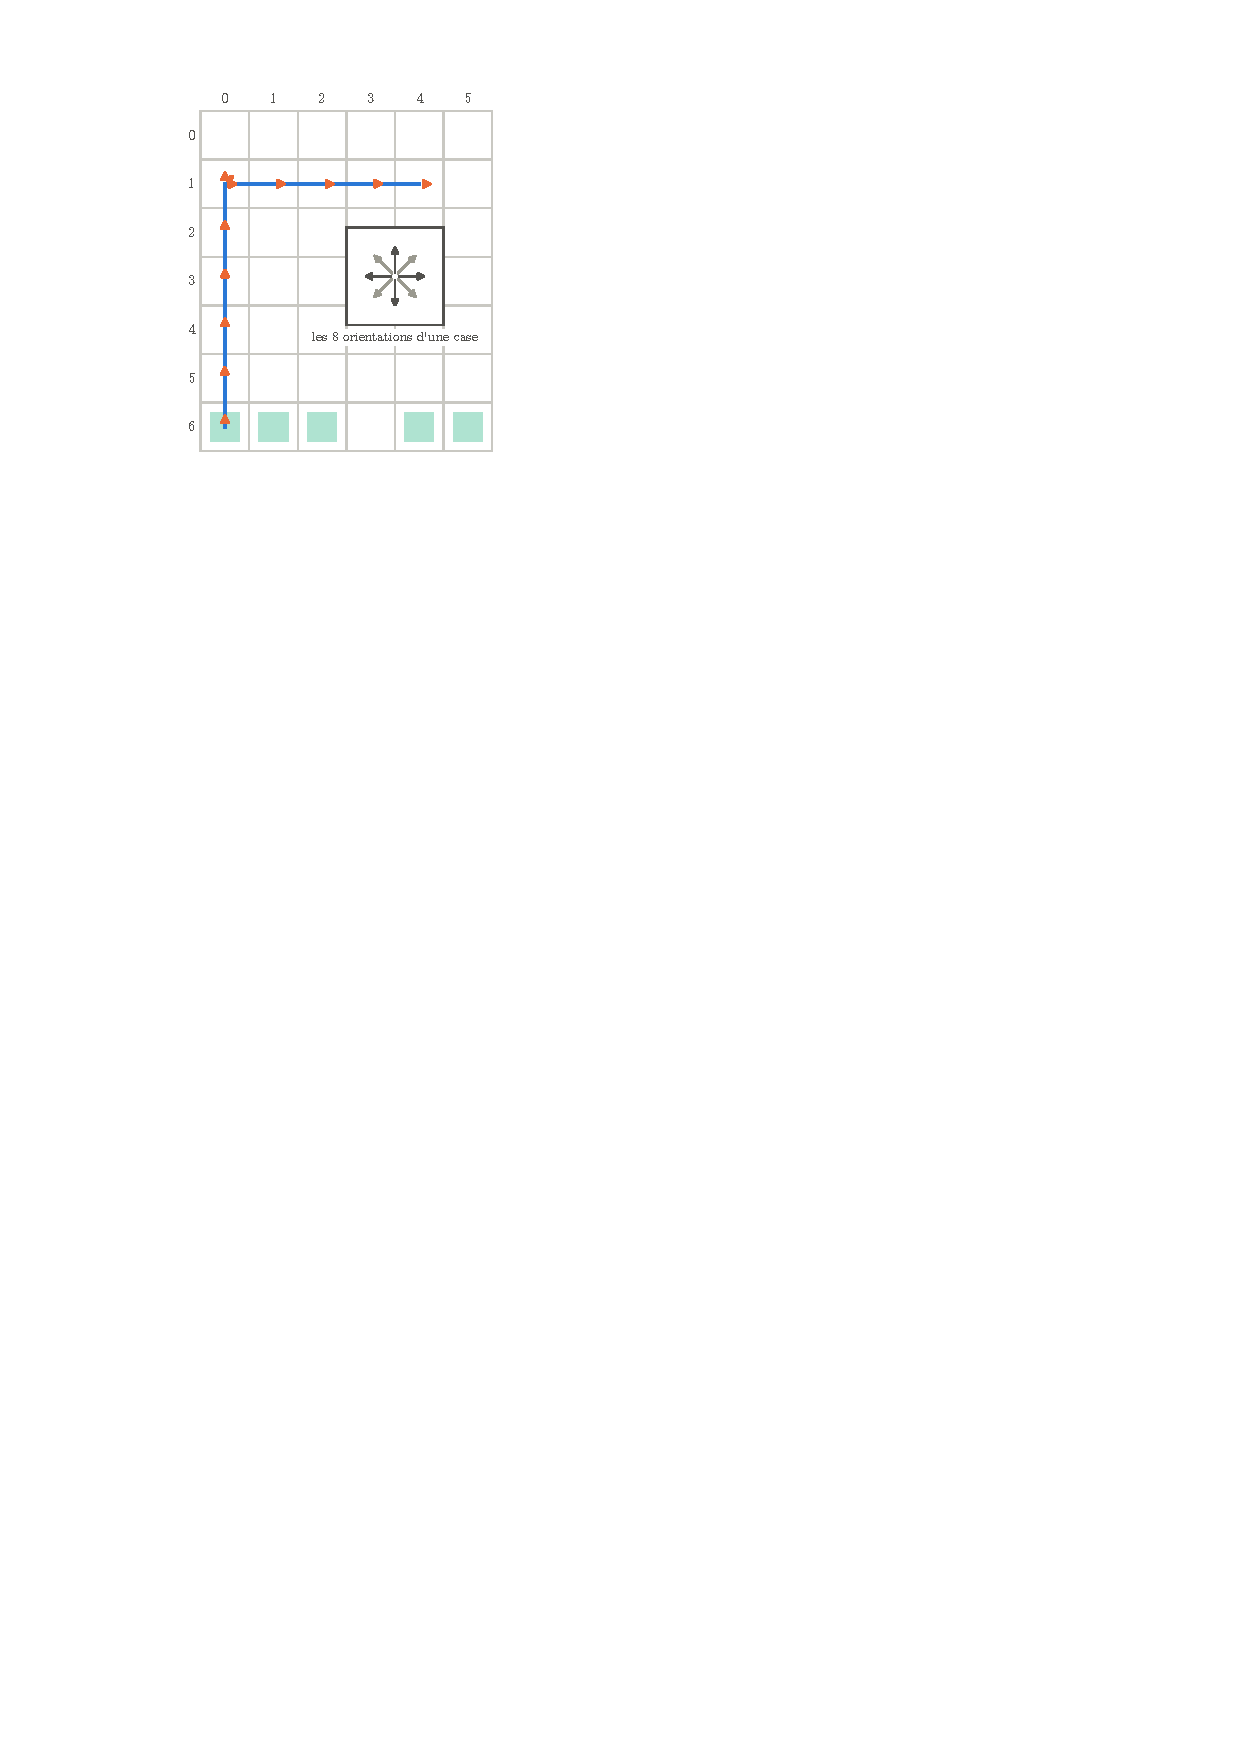
\includegraphics[width=\linewidth]{figs/robot-4}
\caption{Graphe d'états de la planification, avec les indices
de ligne et de colonne du code. Chaque case porte huit orientations. Les cases vertes sont les départs des cinq robots de la
simulation. Le trajet bleu est le plus court chemin calculé par
Floyd-Warshall d'un départ jusqu'à la case (1,\,4), orientation
est, pour un coût de 290.}\label{f:graphe}
\end{figure}

\pa{Graphe d'états.} L'arène de $7 \times 6$ cases est modélisée
par un graphe dont chaque sommet est une case et une
orientation parmi huit, soit 336 états (figure~\ref{f:graphe}). Les arcs
représentent les mouvements possibles : une rotation de
45° coûte 10, une avance d'une case dans l'un des quatre
axes coûte 30, et une capture, qui demande un tour complet, coûte 80. Le graphe compte 814 arcs. L'algorithme
de Floyd-Warshall~\cite{floyd} donne les plus courts chemins entre
toutes les paires d'états en 3~s en Python ; le plus long trajet coûte 410.

\pa{Recherche exhaustive.} Une première approche explorait l'arbre de tous les déplacements possibles des robots
par \en{branch and bound}. L'arbre croît exponentiellement avec le nombre de robots, et les notes du groupe
jugent cette recherche beaucoup trop lente, même après
dix minutes de calcul. Les notes du groupe relèvent la
nature du problème : affecter $n$ robots à $n$ cibles quelconques se résout en temps polynomial par un calcul
de flot, mais imposer à chaque robot sa cible rend le
problème NP-difficile quand on minimise la durée totale de la mission.

\pa{Stratégie gloutonne.} La stratégie retenue suit la planification par priorités~\cite{erdmann,silver}. Chaque robot reçoit une
priorité égale à l'instant où il sera libre, et le robot prioritaire choisit sa prochaine cible en fonction de sa distance
et de l'intérêt de l'état visé. Cet intérêt dépend de la
probabilité d'y voir une balise, estimée à partir des zones
déjà observées et du nombre de balises encore attendues.
Les trajets sont ensuite vérifiés pour éviter les collisions.
Le plan est recalculé dans un \en{thread} séparé dès
qu'une observation nouvelle arrive. Le premier plan pour
cinq robots demande environ 6~s, et les fonctions de base
sur la grille ont été réécrites en C.

Une simulation à cinq robots et douze balises, affichée
avec pygame, a servi à mettre au point la stratégie. Elle
a mis en évidence des situations de \en{deadlock}, où aucun
robot ne trouve de mouvement acceptable, que le code
note comme problème ouvert. Dans notre propre exécution sans affichage, une partie ne s'est pas terminée en cinq minutes.

\section{Résultats et Limites}
Le robot a réussi l'épreuve finale, en exécutant les
ordres du serveur de stratégie et en rapportant ses captures au serveur du cours.

\pa{Odométrie.} Les déplacements reposent sur les seuls
encodeurs, avec un facteur de correction fixe. Toute erreur
de rotation se reporte sur les avances suivantes. Fusionner
l'odométrie et les mesures de la caméra, par exemple avec
un filtre de Kalman, limiterait cette dérive.

\pa{Localisation.} La moyenne des estimations données par
les coins reste sensible à un marqueur mal détecté. Une
vraie triangulation, pondérée par la distance de chaque
marqueur, serait plus robuste.

\pa{Planification.} La stratégie gloutonne répond vite mais
sans garantie, et les \en{deadlocks} restent à traiter. La
planification coopérative avec une table de réservation
espace-temps~\cite{silver} traite précisément ce problème, et le calcul en C de la recherche entière permettrait d'en explorer
davantage dans le même temps.

\section{Conclusion}
Ce projet a mené un robot de son châssis découpé au
Fablab jusqu'à une stratégie collective. Le robot avance
et tourne de façon asservie grâce aux encodeurs, repère et
localise les balises grâce à une caméra calibrée à une fraction de pixel, et suit les ordres d'un serveur de stratégie.
Il a réussi l'épreuve finale. La planification à plusieurs robots, menée en groupe, a montré l'écart entre la recherche
exhaustive, impraticable, et une stratégie gloutonne rapide dont la robustesse reste à améliorer.

{\small
\begin{thebibliography}{9}\setlength{\itemsep}{1pt}
\bibitem{aruco} S. Garrido-Jurado, R. Muñoz-Salinas, F. J. Madrid-Cuevas et M. J. Marín-Jiménez, «~Automatic Generation and Detection of Highly Reliable Fiducial Markers under Occlusion~», \emph{Pattern Recognition}, vol.~47, n\textsuperscript{o}~6, pp.~2280--2292, 2014.
\bibitem{zhang} Z. Zhang, «~A Flexible New Technique for Camera Calibration~», \emph{IEEE Transactions on Pattern Analysis and Machine Intelligence}, vol.~22, n\textsuperscript{o}~11, pp.~1330--1334, 2000.
\bibitem{opencv} G. Bradski, «~The OpenCV Library~», \emph{Dr. Dobb's Journal of Software Tools}, 2000.
\bibitem{astrom} K. J. Åström et R. M. Murray, \emph{Feedback Systems: An Introduction for Scientists and Engineers}, Princeton University Press, 2008.
\bibitem{floyd} R. W. Floyd, «~Algorithm 97: Shortest Path~», \emph{Communications of the ACM}, vol.~5, n\textsuperscript{o}~6, p.~345, 1962.
\bibitem{erdmann} M. Erdmann et T. Lozano-Pérez, «~On Multiple Moving Objects~», \emph{Algorithmica}, vol.~2, pp.~477--521, 1987.
\bibitem{silver} D. Silver, «~Cooperative Pathfinding~», \emph{AIIDE}, AAAI, 2005.
\end{thebibliography}}
\end{document}
